\documentclass[10pt,times,conference,final]{IEEEtran}

\usepackage[latin1]{inputenc}
\usepackage[english]{babel}
\usepackage{graphicx}
%\usepackage{hyperref} %hyperref may not work very well with IEEEtran
\usepackage{cite}
\usepackage{booktabs}
%\usepackage[caption=false,font=footnotesize]{subfig}


\newcommand{\fig}[4][htbp]{
  \begin{figure}[#1] {\centering\scalebox{#2}{\includegraphics{fig/#3}}\par}
    \caption{#4\label{#3}}
  \end{figure}
}

\newcommand{\multfigtwoh}[6][htbp]{
\begin{figure*}[#1]
  \centering
  \subfloat[]{\label{#3}\scalebox{#2}{\includegraphics{fig/#3}}}
  \subfloat[]{\label{#4}\scalebox{#2}{\includegraphics{fig/#4}}}
  \caption{#6}
  \label{#5}
\end{figure*}
}

\newcommand{\multfigtwov}[6][htbp]{
\begin{figure}[#1]
  \centering
  \subfloat[]{\label{#3}\scalebox{#2}{\includegraphics{fig/#3}}}\\
  \subfloat[]{\label{#4}\scalebox{#2}{\includegraphics{fig/#4}}}
  \caption{#6}
  \label{#5}
\end{figure}
}

\newcommand{\figR}[5][htbp]{
  \begin{figure}[#1]{\centering\scalebox{#2}{\includegraphics[angle=#5]{fig/#3}}\par}
    \caption{#4\label{#3}}
  \end{figure}
}

\newcommand{\figTC}[4][htbp]{
  \begin{figure*}[#1] {\centering\scalebox{#2}{\includegraphics{fig/#3}}\par}
    \caption{#4\label{#3}}
  \end{figure*}
}

\newcommand{\figEMPTY}[5][htbp]{
  \begin{figure}[#1]
    \fbox{\begin{minipage}{#2}\hfill\vspace{#3}\end{minipage}}
    \centering
     \label{#4}
    \caption{#5}
  \end{figure}
}

\newcommand{\tab}[3][htbp]{
  \begin{table}[#1]
    \footnotesize
    \centering
    \caption{#3}
    \include{tab/#2}
    \label{#2}
  \end{table}
}

\newcommand{\tabTC}[3][htbp]{
  \begin{table*}[#1]
    \footnotesize
    \centering
    \caption{#3}
    \include{tab/#2}
    \label{#2}
  \end{table*}
}

 %new commands 



\title{High-level Design and Synthesis of a Resource Scheduler}

\author{Jo�o Paulo Pizani Flor,
Tiago Rog�rio M�ck, 
Ant�nio Augusto Fr�hlich\\

\IEEEauthorblockA{Software/Hardware Integration Lab\\
Federal University of Santa Catarina\\
Florian�polis, Brazil\\ 
Email: \{joaopizani,tiago,guto\}@lisha.ufsc.br}
}


\begin{document}
    \maketitle

    \begin{abstract}
        Given the increasing complexity of current embedded systems, hardware design is being
        pushed to a higher level of abstraction, with High-Level Synthesis tools enabling hardware
        synthesis from untimed C++. Still, HLS technology does not provide a clear methodology to derive
        both hardware and software implementations from a single high-level code. This paper describes the
        design, implementation and evaluation of a resource scheduler that has a single C++ description and
        is automatically implementable in both software and hardware.
    \end{abstract}

    \begin{IEEEkeywords}
        High-level synthesis; system-level design; resource scheduling; reconfigurable computing
    \end{IEEEkeywords}

    \section{Introduction}
        %Motivate the usage of higher-level approaches for ES development with the usual
        %time-to-market, complexity, etc. arguments.
        %Motivate unified implementations that can move between software
        %and hardware, to harness parallelism when adequate, design space exploration, etc .
        %Do not talk about hybrid components yet.
        Embedded systems are becoming increasingly complex as the advances of the semiconductor industry
        allow the use of sophisticated computational resources in a wider range of applications. Often, the
        development of such systems encompasses an integrated hardware/software design that can be realized
        by several computer architectures, ranging from 8-bit microcontrollers to complex
        \textit{Multiprocessor Systems-on-Chip}~(MPSoCs). In order to deal with this complexity,
        embedded system designs are being pushed to higher levels of
        abstraction, such as \emph{system-level design}. In this scenario, a convergence between hardware
        and software modeling is desirable, since a unified approach would allow one to decide about 
        hardware/software partitioning later in the design process, maybe even automatically. In the last few
        years, advances in \textit{electronic design automation}~(EDA) tools are allowing hardware synthesis
        from descriptions at the behavioral level \cite{Mentor:Catapult}. These tools allow designers to
        describe hardware components using languages like C++, and with untimed constructs. The focus of
        these tools, however, is hardware synthesis, and they do not provide a clear methodology for
        developing components implementable in hardware and software.

        %Introduce the case study for unified description and implementation (a scheduler).
        %   - Support this choice with two observations:
        %   - A resource scheduler has a fairly complex (asynchronous and autonomous) behavior.
        %   - A hardware-implemented scheduler could (in one possible implementation scenario) have
        %     deterministic execution time, eliminating jitter and allowing hard-real time applications.
        In this paper, we aim to advance in the direction of unified hardware/software design. Previous
        works~\cite{Marcondes:2009} defined guidelines for translating operating system components
        -- such as timers, schedulers, and synchronizers -- from software to hardware and vice versa. These
        components were designed to allow their implementation to migrate between the hardware and software
        domains without the need to modify their client application. Nevertheless, these \emph{hybrid
        components} are defined only in terms of their interface and communication structure, and the
        implementation of their behavior still follows different methodologies. To narrow this gap, we
        describe and evaluate a unified (single-code) resource scheduler. The choice of such component as a
        case study is motivated by its complex behavior. A scheduler may perform operations both
        synchronously (upon request by another component) or asynchronously (by preempting the execution of
        another component). Furthermore, a hardware-implemented scheduler has (in one possible
        microarchitecture) deterministic execution time, eliminating jitter and improving the support of real
        time applications.

        Our design follows the principles defined by the \textit{Application-driven Embedded System Design}
        ~(ADESD)~\cite{Froehlich:2001} methodology. ADESD elaborates on OOP and \textit{Aspect-Oriented
        Programming} concepts, defining a domain engineering strategy focused on the production of
        scenario-independent components. The C++ code of our scheduler leverages on
        \emph{generic programming}~\cite{Czarnecki:2000} techniques such as \emph{static metaprogramming}
        in order to provide an efficient implementation for both hardware and software.

        %The remainder of this paper ir organized as follows...

        %The remainder of this paper is organized as follows: section \ref{section_related_work}
        %discusses related work; section \ref{section_adesd} presents the concepts on which our
        %work is based; sections \ref{section_hybrid_scheduler} and \ref{section_results} 
        %present our approach and the evaluation of our case study; and section 
        %\ref{section_conclusion} closes this paper with our conclusions.
        
    \section{Related work}
        \label{section_related_work}
        %One or two paragraphs:
        % -Talk about related works regarding HW/SW codesign. (see Hugo's papers/thesis
        %  and Tiago's references in Wiki)
        % -Claim that they provide tools and integration/simulation enviroments, but
        %  do not provide a suitable design methodology for the unified design of commands
        %  components.
        %
        %One paragraph:
        % -Talk about HLS tools.
        % -They enable HLS but also do not define a design methodology
        %
        %One or two paragraphs:
        % -ADESD and hybrid components

        %PBD - Metropolis 1 and 2; \cite{Vincentelli:2001,Balarin:2003,Davare:2007}
        %Ptolemy/PeaCE \cite{Eker:2003,Ha:2008} 
        % MPSoC Component Based Desing / ROSES \cite{Cesario:2002,Dziri:2004}        
        Several design methodologies and tools were proposed in order to provide more tightly coupled hardware
        and software design flows ~\cite{Vincentelli:2001,Cesario:2002,Davare:2007}.
        Most of these methodologies are based on the concept of building a system by
        assembling pre-validated components. One example is \emph{Metro-II}~\cite{Davare:2007}. This 
        framework follows the \emph{Platform-based design}~(PDB)~\cite{Vincentelli:2001} methodology, 
        and proposes the use of a metamodel with formal semantics
        that developers can use to capture designs. However, these methodologies do not define clear
        guidelines to design new components which can be reused in a wide range of applications. Also, the
        hardware/software partitioning is defined in the early design phases and is limited by the platform
        specification.

        %HLS for HW-only \cite{Mentor:Catapult}\cite{Fingeroff:2010}
        %FOSSY; \cite{Grimpe:2003}
        %Saturn \cite{Mueller:2010}
        In order to overcome these issues, one must focus on closing the gap between software and hardware
        design. State-of-the-art EDA tools like Catapult C~\cite{Mentor:Catapult} support hardware synthesis
        from high-level C++ constructs, and several works have already demonstrated the applicability of
        high-level synthesis for implementing computation-intense hardware components~\cite{Fingeroff:2010}.
        The OSSS+R methodology \cite{Grimpe:2003} advances further and aims at generating both hardware and software from
        the same description. It raises the level of abstraction of RTL SystemC by adding language constructs to
        support polymorphism and high-level communication. However, hardware/software partitioning must still
        be done early in the design process\cite{Gruttner:2008}, and the inclusion of non-standard language
        constructs reduces compatibility with available compilers and synthesis tools. The \emph{Saturn}
        \cite{Mueller:2010} design flow also contributes in this direction, but follows a different approach.
        The authors propose \emph{SysML}, an extension of UML for system-level design, and a tool which
        generates C++ for software and RTL SystemC for hardware. However, Saturn has the same limitations
        described previously: hardware and software cannot be generated from the same specification.
        Additionally, it is not clear whether their tool generates code only for the interface and
        integration of components, or the behavior is also implemented in SysML.

        The ADESD~\cite{Froehlich:2001} methodology elaborates on commonality and variability analysis to add
        the concept of aspect identification and separation at early stages of design. It defines a domain
        engineering strategy focused on the production of families of scenario-independent components.
        Dependencies observed during domain engineering are captured as different aspects, thus enabling
        components to be reused on a variety of execution scenarios with the application of proper aspects.
        In \cite{Marcondes:2009} ADESD's design artifacts were explored to define guidelines for the development
        of components which could migrate between the hardware and software domains, and a common architecture for
        communication between components living in hardware and/or software. These \emph{hybrid components}
        provide more flexibility and allow for the postponement of the hardware/software partitioning.
        However, hybrid components still require duplicated descriptions (in a software programming language
        and in a hardware description language). In the next sections we demonstrate how ADESD's design artifacts
        can be used to overcome such limitations through the unified (single code) design of a hybrid
        hardware/software resource scheduler.
        
        %These design artifacts can be implemented in C++ by leveraging on 
        %\emph{generic programming}~\cite{Czarnecki:2000} techniques such as \emph{static metaprogramming}
        %in order to achieve high reusability with low overhead.
        % Mention EPOS as THE EXAMPLE of ADESD, using static metaprogramming (C++ templates) to achieve
        % ADESD's goals.
    
    \section{Development and implementation of a hybrid HW/SW resource scheduler}
        \label{section_hybrid_scheduler}
        %TODO
        % * Show that the design of the EPOS Scheduler abstraction facilitates our approach (separating
        % the execution scenario from the functionality). Features such as interrupt generation and
        % context switch are not part of the scheduler itself.
        As a case study we chose to modify the scheduler of the EPOS operating system\cite{Froehlich:2001},
        making its C++ code unified and suitable for automatic implementation in both hardware and
        software. EPOS's domain engineering simplified our work by providing a good
        \emph{separation of concerns} around the scheduler. Figure \ref{fig:scheduling-classes}
        shows a simplified class diagram of the scheduling-related classes in EPOS.
        \begin{figure}[h]
            \begin{center}
                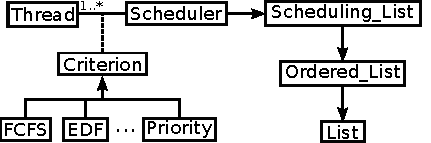
\includegraphics[width=0.9\columnwidth]{fig/scheduler-structures.pdf}
            \end{center}
            \caption{Simplified class diagram of scheduling-related classes in EPOS.}
            \label{fig:scheduling-classes}
        \end{figure}

        The Scheduler class is responsible only for keeping ordered queues, with the ordering defined by the
        scheduling criterion. An object of the Scheduler class also allows its callers to insert and remove
        clients from the queues, as well as to get the current and next owners of the resource. In our case
        study, we implemented a scheduler for threads. However, the Scheduler code is largely independent of
        the type of resource being scheduled (in fact, Scheduler is a \emph{class template}). Furthermore,
        concerns such as timing interrupt generation and context switching are handled by other classes
        (Alarm and CPU, respectively).

        Among all classes in figure \ref{fig:scheduling-classes}, we adapted the code of the Scheduler class
        (also of its base classes), so that it can now serve as input for both hardware and software
        implementation flows. Figure \ref{fig:flows} summarizes both flows.
        \begin{figure}[h]
            \begin{center}
                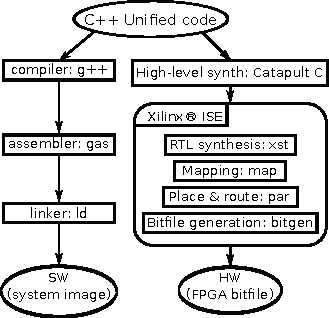
\includegraphics[width=0.7\columnwidth]{fig/implementation-flows.pdf}
            \end{center}
            \caption{Implementation steps and tools used, for both HW and SW flows.}
            \label{fig:flows}
        \end{figure}

        An important consideration about figure \ref{fig:flows} is that the usage of a unified code for the
        scheduler did not affect the software implementation flow. The toolchain consists only of standard
        open-source tools, and is \emph{exactly the same} as the one used with the software-only code. In the
        hardware implementation flow, the only notable addition is the \emph{High-level synthesis} step, done
        by Catapult C of Mentor Graphics\textregistered . Catapult C takes untimed C++ as input, performs
        technology mapping, resource allocation and scheduling, producing as its result a RTL (VHDL or
        Verilog) description of the hardware block.

        % List the limitations imposed by the high-level synthesis flow
        During our initial attempts at high-level synthesis we were faced with three fundamental limitations
        imposed by the toolchain, and these limitations have guided our development from the very beginning.
        They are, namely:
        \begin{enumerate}
            \item Pointers have no intrinsic meaning in hardware. They are mapped to indices
                of the storage structures to which they point. Thus, \emph{no null or otherwise invalid
                pointers} are allowed in the source code.
            \item There is no feature similar to dynamic memory allocation in hardware. Therefore, in a
                \emph{synthesizable} code, all data structures must reside in statically allocated memory.
            \item The top-level interface of the resulting hardware block (port directions and sizes) is
                inferred by Catapult C from a \emph{single function signature}. There must be only one
                function in the code with the pragma ``hls\_design top''.
        \end{enumerate}

        % Mention the Maybe<T> changes to the C++ scheduler code
        % * The few modifications necessary to the old software-only scheduler code are well-understood
        % structures (option type) and these modifications cause an INSIGNIFICANT change in runtime
        % performance of the code when executing in software. The detailed comparison and analysis is done
        % in the results section.
        Limitation number 1 influenced our development deeply, mainly because several methods of the Scheduler
        class used null pointers to report failures. To overcome this limitation, we changed the code of the
        scheduler (and of its internal data structures) to utilize an \emph{option type}.

        An option type is a container for a generic value, and has an internal state which represents the
        presence or absence of this value. Option types are very popular in functional programming as the
        return type of functions that can fail. We implemented an option type in the C++ class template
        \emph{Maybe\textless T\textgreater}, which has the following constructors:
        \begin{verbatim}
Maybe(): _exists(false), _thing(T()){}
Maybe(T obj): _exists(true), _thing(obj){}
        \end{verbatim}
        One constructor represents the absence of a value in the container while the other represents its
        presence. By replacing all occurrences of simple pointers (T*) in the scheduler code with
        Maybe\textless T*\textgreater values, we completely avoided passing invalid pointers around. Still,
        the modified code was not significantly larger, neither did it run significantly slower, as we
        clarify in section \ref{section_results}.

        The other two limitations of the hardware flow (no dynamic memory and a single function as interface)
        were overcome by \emph{wrapping} the scheduler code with two C++ class templates: they are
        responsible, respectively, for storage allocation and method call dispatch. The functionality and
        architecture of these wrappers are summarized in figure \ref{fig:wrappers}.
        \begin{figure}[ht]
            \begin{center}
                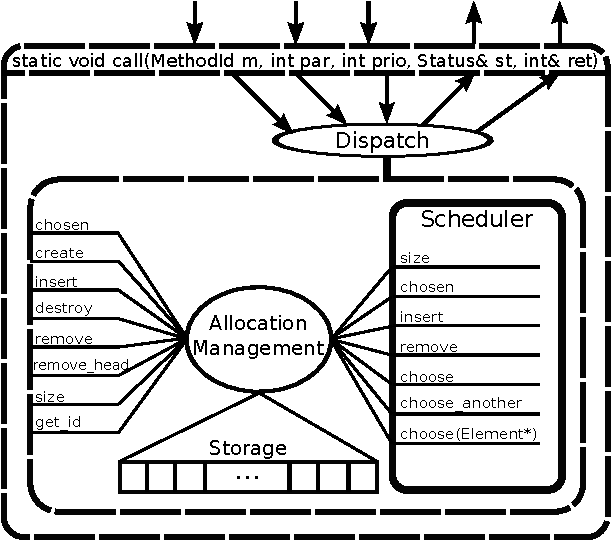
\includegraphics[width=0.87\columnwidth]{fig/scheduler-wrappers.pdf}
            \end{center}
            \caption{Wrappers that adapt the Scheduler class to make it synthesizable.}
            \label{fig:wrappers}
        \end{figure}

        % * Emphasize that the lowest layer (core) of this architecture is EXACTLY
        % the same code that runs in software.
        The innermost block in the ``onion-like'' architecture of figure \ref{fig:wrappers} is the
        Scheduler C++ class template. This exact code serves as input to the software implementation flow.
        The two wrappers mentioned beforehand are represented by the two outermost blocks in the diagram,
        with dashed bounding boxes.
        
        In figure \ref{fig:wrappers}, we can also see that the interface of the storage allocation
        wrapper is largely the same as the interface of the Scheduler class. The only responsibility
        of the storage allocator is, therefore, to provide storage space -- reserving and releasing
        it on demand -- to the wrapped Scheduler instance.
        
        The interface of the dispatch wrapper is radically different, however, and has a single
        function with all input and output parameters used by the wrapped class. One notable
        parameter of type \emph{MethodId} is present in the call function of the dispatch wrapper.
        The responsibility of the dispatch wrapper is to interpret the value of this parameter, perform the
        necessary type conversions and call the appropriate method of the wrapped class. The value returned
        by the called method is also inspected, converted if necessary and assigned to one of the
        wrapper's output parameters.

        %% Comment on genericity of the wrappers (both are highly parameterized class templates)
        Both wrappers developed are highly generic and were purposefully designed to be able to wrap other
        components. In fact, they are C++ class templates, parametrized by the wrapped class and the size of
        the pre-allocated storage space.


    \section{Results}
        \label{section_results}
        Our hybrid implementation of a resource scheduler was evaluated in both software and hardware-based
        scenarios. The high-level synthesis of the scheduler was performed using Catapult-C\textregistered ,
        from Mentor Graphics, and for the RTL synthesis and translation we used the ISE toolchain, from
        Xilinx\textregistered . The following three hardware microarchitectures were investigated:
        \begin{enumerate}
            \item \emph{Fully automatic} microarchitecture: The complete synthesis process, from untimed C++
                to FPGA bitfile, happened with no human interaction. All directives and flags were left at
                their default values.
            \item \emph{Fully serial} microarchitecture: Catapult C was instructed to map data structures in
                the C++ code to memories (BRAMs). Our goal in this case was to save device area.
            \item \emph{Fully parallel} microarchitecture: Data structures were mapped to registers and all
                loops were unrolled, in order to fully harness the available parallelism in the algorithms.
        \end{enumerate}

        % ** We compare the several microarchitectures generated from the unified description among themselves
        % and with the handwritten RTL scheduler (\cite{Marcondes:2009}).
        We evaluated the performance of all three automatically-generated microarchitectures by comparing
        them (both in terms of area and critical path delay) with a handwritten RTL scheduler implementation
        \cite{Marcondes:2009:2}. All implementations were synthesized targeting a Virtex6 (XC6VLX240T) device
        from Xilinx\textregistered , and with a target clock frequency of 50MHz. Table \ref{tab:results-hw}
        summarizes the performance of all evaluated hardware microarchitectures, both generated and
        handwritten.
        \begin{table}[h]
    \begin{center}
        \begin{tabular}{cccc}
            \toprule
            \textbf{Scenario} & \textbf{LUTs} & \textbf{Device occupation} & \textbf{Max. delay}
            \tabularnewline
            \midrule
            Handwritten RTL  & 1250  & 0.83\%   &  5.598 ns
            \tabularnewline
            Fully serial     & 1654  & 1.10\%   &  6.672 ns
            \tabularnewline
            Fully automatic  & 3392  & 2.25\%   &  7.341 ns
            \tabularnewline
            Fully parallel   & 5121  & 3.40\%   &  10.597 ns
            \tabularnewline
            \bottomrule
        \end{tabular}
    \end{center}
    \caption{Performance summary of all evaluated HW microarchitectures}
    \label{tab:results-hw}
\end{table}


        % * Emphasize the most interesting (opposite) synthesis scenarios:
        % ** The completely serial scenario (implemented with BRAMs) gets VERY CLOSE to the handwritten RTL in
        % terms of area.
        % ** The completely parallel scenario provides completely deterministic execution time, constant and
        % the same (worst-case) for all operations.
        Particularly interesting is the fully serial generated microarchitecture, which gets close to the
        handwritten RTL, both in terms of area (+32\%) and of maximum delay (+19\%). Furthermore, despite
        having greater area and maximum delay, the fully parallel microarchitecture also has its
        advantage: all operations (search, insert, remove, etc.) are done in parallel, and therefore
        within a constant number $ n $ of cycles, which is the same for all operations. This eliminates
        jitter in scheduling, improving the support of hard real-time applications.

        % ** We compare the old software-only C++ source-code of the scheduler with the new unified
        % implementation in terms of execution time and code size.
        As already mentioned in section \ref{section_hybrid_scheduler}, we changed the
        original C++ source code of the scheduler (by introducing the option type) in order to make
        it synthesizable. The introduction of the option type happened in the unified code, affecting,
        therefore, also the software implementation.

        To measure the effect of these changes, we compared the old (software-only) C++ scheduler
        code with the unified one, in terms of code size and execution time. We chose MIPS32 as the
        target architecture for compilation, and measured the resulting EPOS system image size and
        the execution time of some methods for both scheduler implementations.
        Table \ref{tab:results-sw} summarizes these results.
        \begin{table}[h]
    \begin{center}
        \begin{tabular}{cccc}
            \toprule
            \textbf{Metric} & \textbf{SW-only} & \textbf{Unified} & \textbf{difference}
            \tabularnewline
            \midrule
            Code size                     & 29580 B                 & 29700 B                 & 0.41\%
            \tabularnewline
            \emph{insert} execution time  & 51 $\times 10^{-1}\mu$s & 53 $\times 10^{-1}\mu$s & 3.92\%
            \tabularnewline                                           
            \emph{remove} execution time  & 27 $\times 10^{-1}\mu$s & 29 $\times 10^{-1}\mu$s & 7.41\%
            \tabularnewline                                           
            \emph{suspend} execution time & 32 $\times 10^{-1}\mu$s & 34 $\times 10^{-1}\mu$s & 6.25\%
            \tabularnewline                                           
            \emph{resume} execution time  & 42 $\times 10^{-1}\mu$s & 43 $\times 10^{-1}\mu$s & 2.38\%
            \tabularnewline                                           
            \emph{choose} execution time  & 61 $\times 10^{-1}\mu$s & 67 $\times 10^{-1}\mu$s & 9.84\%
            \tabularnewline
            \bottomrule
        \end{tabular}
    \end{center}
    \caption{Comparison of generated code size and execution time between SW-only and unified
        scheduler versions}
    \label{tab:results-sw}
\end{table}


        The execution time measurements were done by instrumenting Scheduler methods with calls to a
        \emph{timestamp counter} that runs at the same frequency as the CPU. The resolution, therefore, is 20
        ns, and our measurements are in tenths of microseconds. A dining philosophers application was used to
        request the scheduler's services. We took 100 sample runs of this application, and table
        \ref{tab:results-sw} shows the average execution times of the methods.


    \section{Conclusion}
        \label{section_conclusion}
        %TODO
        % * Claim that the decisive factor in allowing our unified description is EPOS modelling following
        % ADESD, and that our ``hardware scenario adapters'' follow the same approach.
        In this paper we presented the unified design and implementation of a generic resource scheduler. The
        exact same C++ source code serves as input for both the hardware and software implementation flows.
        Furthermore, the performance of this unified code in software and hardware execution scenarios is
        close to the performance of software-only and hardware-only implementations, respectively. No
        additional tools were necessary to generate a software system image from the unified code, and the
        adaptions necessary to hardware synthesis were organized in a layered architecture, facilitating
        automatic application.

        Careful domain engineering and system design leads to algorithm implementations that are largely
        separated from execution scenario details. Our case study shows that code following these guidelines
        (specially the ADESD methodology, as presented in section \ref{section_related_work}) is suitable for
        automatic implementation in both hardware and software scenarios. During the development of
        the hardware scenario adapters, we came
        across the hypothesis that these adapters could be modeled as aspects\cite{Czarnecki:2000}. The
        further investigation of this hypothesis constitutes important future work related to the research
        exposed in this paper.
        % * All modifications (option type) and layers that we needed to add to the C++ source code of the
        % scheduler SEEM TO FIT the definition of an aspect.

        % * Our design facilitates design space exploration, by allowing the system engineer to effectively
        % POSTPONE design choices related to the actual device where the algorithm will execute.
        As a last remark we emphasize the fact that programming algorithms using unified source code,
        as we proposed, facilitates design space exploration through two mechanisms:
        \begin{itemize}
            \item Design choices regarding execution scenario (whether hardware or software) can be
                \emph{postponed}, with two advantages: duplicated testbenches are avoided, and the
                fine-tuning of parameters can be done in the unified code.
            \item The automatic derivation of hardware from the unified code is guided by \emph{synthesis
                directives}, which can be optimized by design space exploration frameworks.
        \end{itemize}
        

    \bibliographystyle{IEEEtran}
    \bibliography{paper}

\end{document}
